\documentclass{article}
\usepackage[utf8x]{inputenc}
\usepackage{ucs}
\usepackage{amsmath} 
\usepackage{amsfonts}
\usepackage{upgreek}
\usepackage[english,russian]{babel}
\usepackage{graphicx}
\usepackage{float}
\usepackage{textcomp}
\usepackage{hyperref}
\usepackage{mathtools}
\usepackage{geometry}
  \geometry{left=2cm}
  \geometry{right=1.5cm}
  \geometry{top=1cm}
  \geometry{bottom=2cm}
\usepackage{tikz}
\usepackage{ccaption}
\usepackage{multicol}
\usepackage{listings}

\DeclarePairedDelimiter\ceil{\lceil}{\rceil}
\DeclarePairedDelimiter\floor{\lfloor}{\rfloor}

\begin{document}
\pagenumbering{gobble}

\lstset{
  language=C,                % choose the language of the code
  basicstyle=\linespread{1.1}\ttfamily,
  columns=fixed,
  fontadjust=true,
  basewidth=0.5em,
  keywordstyle=\color{blue}\bfseries,
  commentstyle=\color{gray},
  stringstyle=\ttfamily\color{orange!50!black},
  showstringspaces=false,
  %numbers=false,                   % where to put the line-numbers
  numbersep=5pt,
  numberstyle=\tiny\color{black},
  numberfirstline=true,
  stepnumber=1,                   % the step between two line-numbers.        
  numbersep=10pt,                  % how far the line-numbers are from the code
  backgroundcolor=\color{white},  % choose the background color. You must add \usepackage{color}
  showstringspaces=false,         % underline spaces within strings
  captionpos=b,                   % sets the caption-position to bottom
  breaklines=true,                % sets automatic line breaking
  breakatwhitespace=true,         % sets if automatic breaks should only happen at whitespace
  xleftmargin=.2in,
  extendedchars=\true,
  keepspaces = true,
}
\lstset{literate=%
   *{0}{{{\color{red!20!violet}0}}}1
    {1}{{{\color{red!20!violet}1}}}1
    {2}{{{\color{red!20!violet}2}}}1
    {3}{{{\color{red!20!violet}3}}}1
    {4}{{{\color{red!20!violet}4}}}1
    {5}{{{\color{red!20!violet}5}}}1
    {6}{{{\color{red!20!violet}6}}}1
    {7}{{{\color{red!20!violet}7}}}1
    {8}{{{\color{red!20!violet}8}}}1
    {9}{{{\color{red!20!violet}9}}}1
}

\section*{Хеш-таблицы: Домашнее задание}

\begin{center}
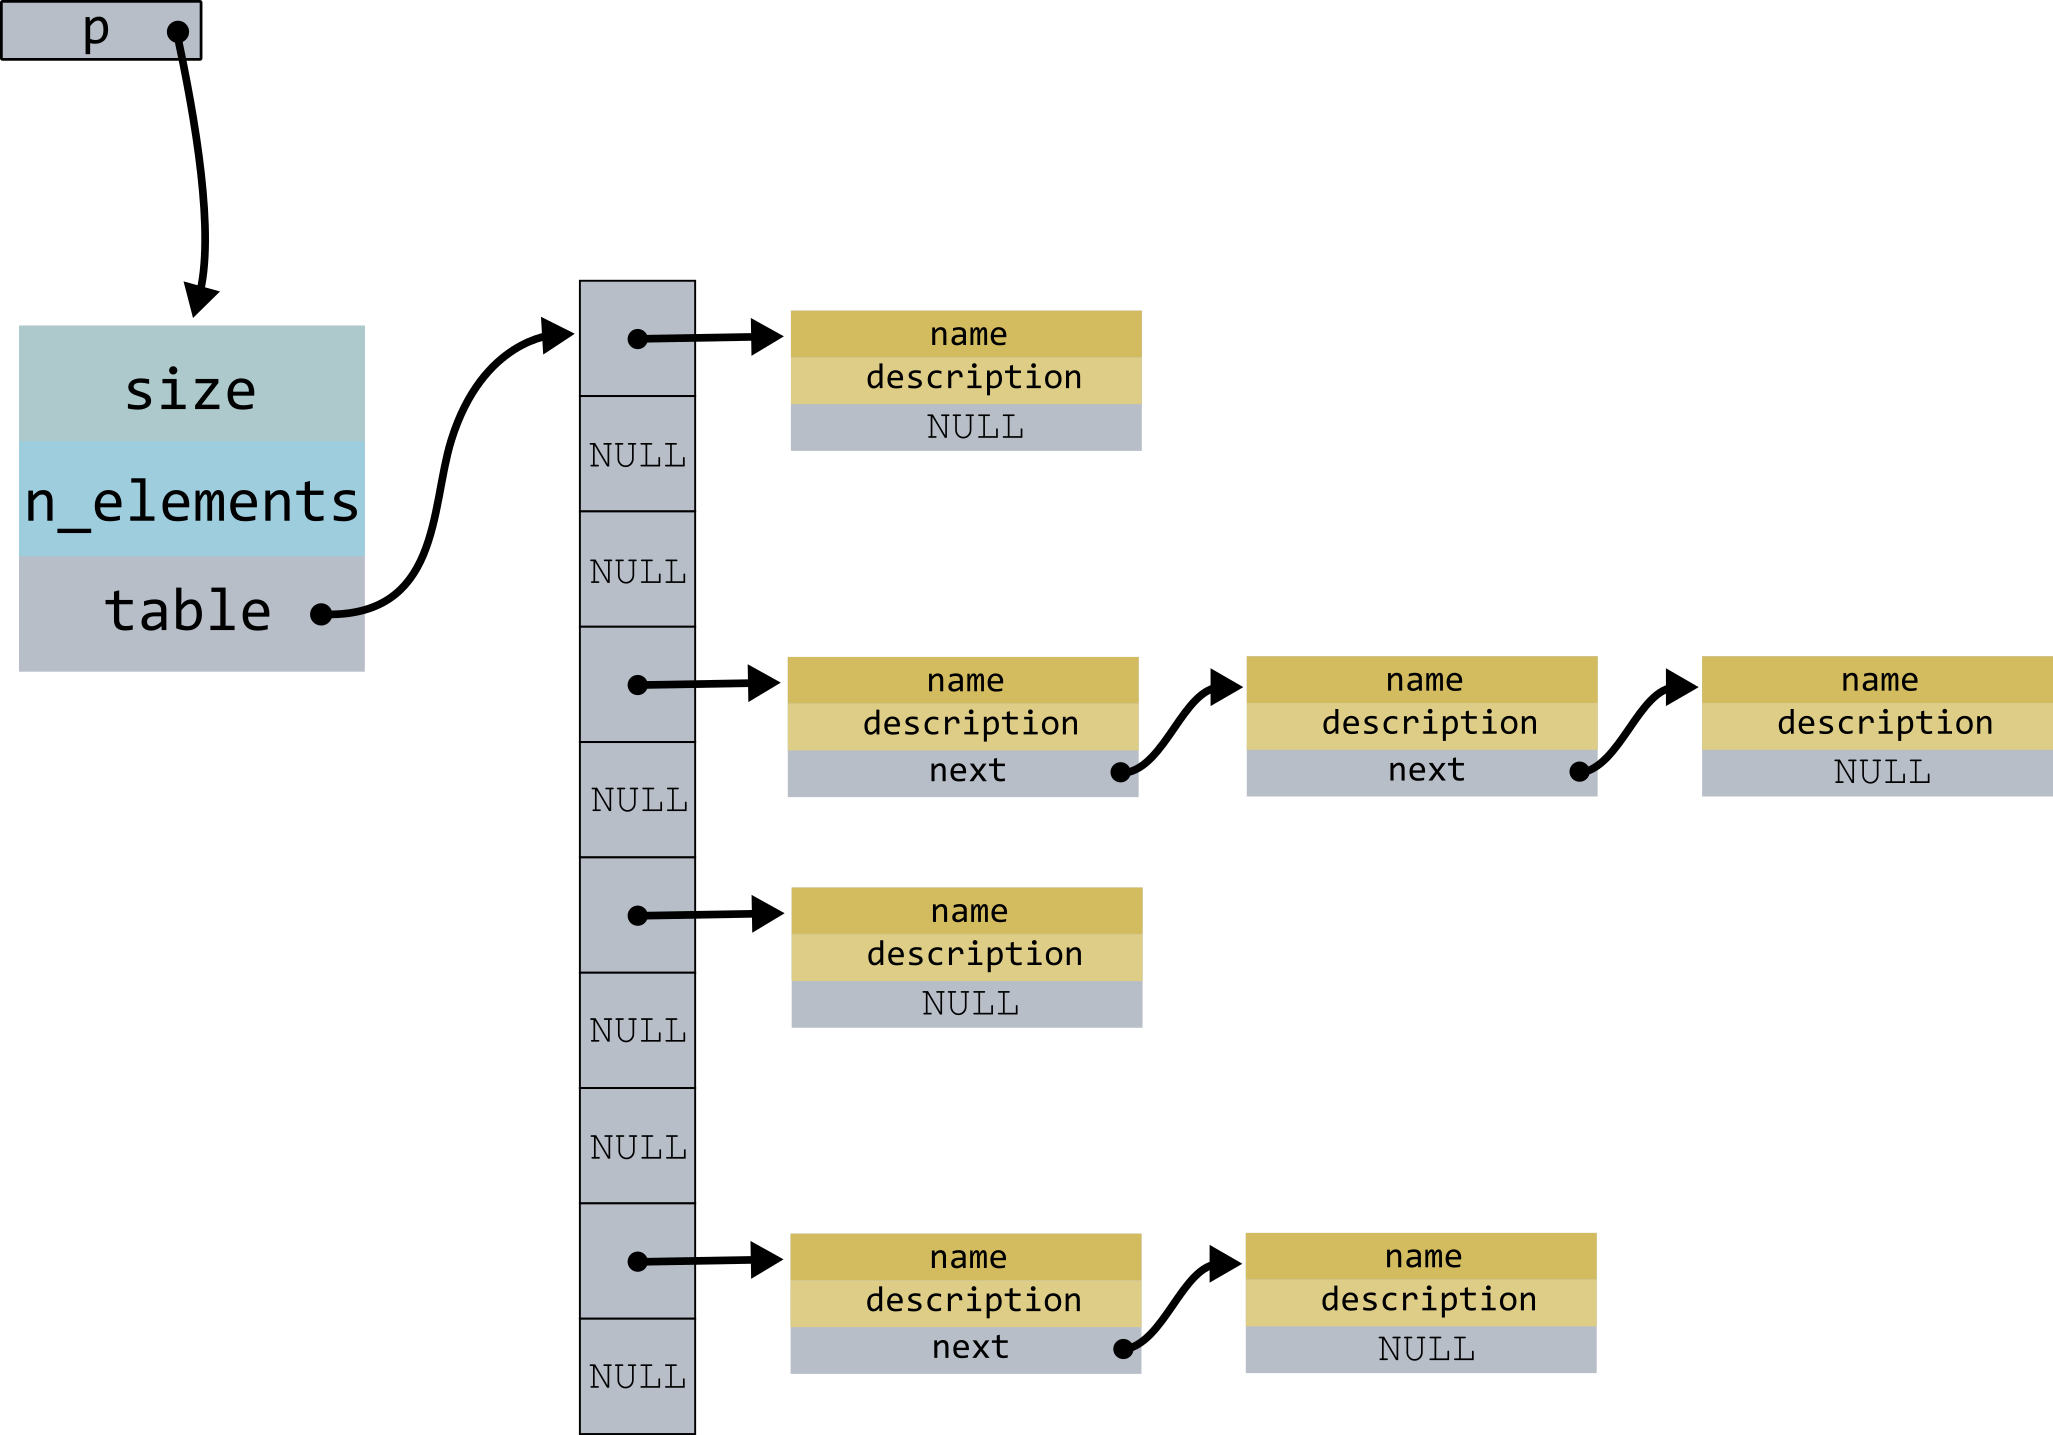
\includegraphics[scale=0.85]{../images/hashtable.png}
\end{center}

В файле \texttt{hash.c} лежит реализация хеш-таблицы (решение задач с классного занятия).
\section*{Задачи:}
\begin{itemize}
\item \textbf{Перестройка таблицы:} Видоизмените функцию \texttt{hashtable\_insert} так, чтобы она проверяла загруженность таблицы при каждом добавлении элемента. Если загруженность таблицы больше чем \texttt{MAX\_LOAD\_FACTOR}, то таблица должна будет вырасти в \texttt{GROWTH\_FACTOR} раз. При этом положения каждого элемента таблицы могут измениться. Проще всего создать новую таблицу и добавить туда все элементы из старой.
\item \textbf{Множество:} Абстрактный тип данных множество (Set) - это некоторая коллекция элементов с определёнными операциями:
	\begin{itemize}
	\item \texttt{insert(S, x)} - добавляет элемент \texttt{x} в множество \texttt{S}; если элемент уже есть, то ничего не делает.
	\item \texttt{erase(S, x)} - удаляет элемент \texttt{x} из множества \texttt{S}; если такого элемента нет, то ничего не делает.
	\item \texttt{is\_element\_of(x, S)} - проверяет входит ли элемент \texttt{x} в множество \texttt{S}.
	\end{itemize}
Конечно, этот абстрактный тип данных можно реализовать с помощью простого массива или связного списка, но при этом операции над множеством будут занимать время $O(n)$, что очень долго. Поэтому множество реализуется с помощью хеш-таблицы $O(1)$, либо с помощью сбалансированного дерева $O(log(n))$. 
В этом задании вам нужно реализовать множество, хранящее целые числа, с помощью хеш-таблицы. Помимо операций \texttt{insert}, \texttt{erase}, \texttt{is\_element\_of}, нужно будет написать функции \texttt{create}, \texttt{print} и \texttt{destroy}. \\
Пример работы с таким множеством (этот код должен напечатать \texttt{NO}):
\begin{multicols}{1}
\begin{lstlisting}
Set* s = set_create();
set_insert(s, 15);
set_insert(s, 4);
set_insert(s, 15);
set_insert(s, 42);
set_erase(s, 15);



if (is_element_of(15, s))
	printf("YES\n");
else
	printf("NO\n");
set_destroy(s);


\end{lstlisting}
\end{multicols}
\item \textbf{Уникальное число:} В файле \texttt{special\_numbers.txt} лежит набор из 20001 чисел. Почти все числа из этого набора встречаются парами (содержатся в наборе чётное число раз). Но в наборе есть одно уникальное число, которое встречается лишь один раз. Найдите это число. \\
Напоминание как считать числа из файла на C:
\begin{lstlisting}
int main()
{
	FILE* file = fopen("special_numbers.txt", "r");
	int N;
	int array[20001];
	fscanf(file, "%d", &N);
	for (int i = 0; i < N; i++)
		fscanf(file, "%d", &array[i]);

}
\end{lstlisting}
Файл \texttt{special\_numbers.txt} должен лежать в той же папке, что и \textit{запускаемый исполняемый файл} (если вы используете IDE, то это не обязательно та папка в которой у вас лежит исходный код).
\item \textbf{Словарь:} Ассоциативный массив или словарь (англ. dictionary или map или associative array) является важнейшим абстрактным типом данных в программировании. Он представляет собой коллекцию пар \texttt{<ключ, значение>} с определёнными следующими операциями:
	\begin{itemize}
	\item \texttt{insert(M, key, value)} - вставляет в словарь \texttt{M} пару \texttt{<key, value>}. Если элемент с таким ключом уже есть, то ничего не делает.
	\item \texttt{assign(M, key, value)} - вставляет в словарь \texttt{M} пару \texttt{<key, value>}. Если элемент с таким ключом уже есть, то устанавливает новое значение у этого ключа.
	\item \texttt{erase(M, key)} - удаляет из словаря \texttt{M} пару с ключом \texttt{key}. Если элемента с таким ключом нет, то ничего не делает.
	\item \texttt{find(M, key)} - ищет в словаре \texttt{M} пару с ключом \texttt{key}. (функция, соответствующая этой операции, должна возвращать указатель на элемент или \texttt{NULL}, если такого элемента нет)
	\end{itemize}

Обычно словарь реализуется с помощью хеш-таблицы, либо с помощью сбалансированного дерева. И ключ и значение может быть переменной любого типа. Словарь с точки зрения интерфейса можно рассматривать как массив у которого в качестве индекса может выступать значения любых типов, а не только целых чисел.\\
По сути, в классной задаче мы создали славарь, у которого в качестве и ключа и значения были строки.
В этой задаче вам нужно реализовать словарь, у которого в качестве ключа будет строка, а в качестве значения - целое число. \\
Пример работы с таким словарём (пара город - численность населения):

\begin{lstlisting}
int main()
{
	Map* m = map_create();
	map_insert(m, "Dolgoprudny", 90956);
	map_insert(m, "London", 8908081);
	map_insert(m, "Montevideo", 1719453);
	map_assign(m, "Adelaide", 1345777);
	map_assign(m, "Dolgoprudny", 108861); // Как бы m["Dolgoprudny"] = 108861;

	Node* p = map_find(m, "London");
	if (p != NULL)
		printf("London is in the map. Population = %d\n", p->value);
	else
		printf("No London in the map\n");
	map_destroy(m);
}
\end{lstlisting}
\end{itemize}
\end{document}
